% \begin{flushright}
%   \makebox[\textwidth]{
\includegraphics[width=0.4\paperwidth, left, height=0.2\paperheight]{imagenes/zombieland.jpg}}
% \end{flushright}
\begin{figure}[h]
\begin{center}

\includegraphics[width=0.6\textwidth] {imagenes/zombieland.png}
\end{center}
\end{figure}

\subsection{Problema a resolver}

El problema a resolver consiste en salvar la mayor cantidad de ciudades de la invasión zombie. Para lograr tal fin, se busca lanzar un ataque coordinado, utilizando los soldados que ya estan en cada ciudad y enviando refuerzos a las mismas, cuya cantidad esta limitada por el presupuesto inicial. 

Para salvar una ciudad la proporción zombie-soldado debe ser de, al menos, 1 soldado por cada 10 zombis. La cantidad de zombis y soldados de cada ciudad es conocida, como también el costo de enviar un soldado a la misma.

Se busca un algoritmo que, tomando el estado actual de todas las ciudades del país, y un presupuesto, optimize el envio de soldados a cada ciudad para salvar la mayor cantidad de ciudades, detallando cuantas ciudades son salvadas y cuantos soldados se envía a cada ciudad del país.

\begin{itemize}
\item Ejemplo: Situación inicial.

\begin{codesnippet}
5 ciudades, $ 600 presupuesto
ciudad 1: 10 zombis 2 soldados $ 500 costo p/soldado
ciudad 2: 20 zombis 2 soldados $ 400 costo p/soldado
ciudad 3: 30 zombis 2 soldados $ 300 costo p/soldado
ciudad 4: 40 zombis 2 soldados $ 200 costo p/soldado
ciudad 5: 50 zombis 2 soldados $ 100 costo p/soldado
\end{codesnippet}
\item Solución del ejemplo:

\begin{codesnippet}
4 ciudades salvadas (todas menos la 4) 
ciudad 1: 0 soldados enviados (salvada, $ 0 costo)
ciudad 2: 0 soldados enviados (salvada, $ 0 costo)
ciudad 3: 1 soldados enviados (salvada, $ 300 costo)
ciudad 4: 0 soldados enviados (no es salvada, $ 400 costo)
ciudad 5: 3 soldados enviados (salvada, $ 300 costo)
\end{codesnippet}
\end{itemize}

\subsection{Resolución planteada}

La solución planteada utiliza la \texttt{técnica algorítmica golosa}. La idea de la misma es ordenar las ciudades en orden creciente en un vector según el \texttt{costo de salvar} cada ciudad e ir recorriendo el vector restando al presupuesto disponible ($P$) \texttt{el costo de salvar} cada ciudad, hasta que el mismo se agote o todas las ciudades sean salvadas, guardando en un contador la cantidad de ciudades salvadas y en un vector del mismo tamaño que la cantidad de ciudades ($n$), en el \texttt{indice de la ciudad}, los \texttt{soldados a enviar} a cada ciudad (este vector es inicializado en 0) . El \texttt{costo de salvar} cada ciudad se calcula a partir de $\lceil \frac{z}{10} \rceil$, donde $z$ es la cantidad de zombis en la ciudad, restándole a ese resultado la cantidad de soldados ($s$) en la ciudad, y por último, multiplicar el resultado previamente obtenido por el costo de enviar refuerzos ($c$) a la ciudad. En caso de que ese valor sea negativo, se pone en 0. La cantidad de \texttt{soldados a enviar} se calcula de la misma manera que el \texttt{costo de salvar} cada ciudad, sin hacer la ultima multiplicación. El \texttt{indice de la ciudad} se refiere al renglón en donde aparece la ciudad en el input. Por último se imprime por pantalla el contador de ciudades salvadas y el vector que contiene los \texttt{soldados a enviar}.
En pseudocódigo:
\newline \newline
\begin{codesnippet}
Creamos un vector infoCiudad de tamaño igual a n.
Creamos un vector soldadosPorCiudad de tamaño n, inicializado en 0.
Para cada ciudad: 
	Tomamos su z, s y c, y
	Hacemos soldados a enviar = parte alta de la división z / 10  - s 
	costo de salvar = soldados a enviar * c,
	Si costo de salvar es menor a 0, 
    	     Hacemos soldados a enviar y costo de salvar = 0.
        Insertamos cada ciudad en el vector infoCiudad
Ordenamos el vector infoCiudad segun costo de salvar.
Para todo i desde 1 hasta n:
 	Si P es mayor o igual al costo de salvar la i-ésima ciudad 
  		Incrementamos el contador de ciudades salvadas
  		Guardamos en soldadosPorCiudad[i] la cantidad de soldados a enviar
        	  Hacemos P = P - costo de salvar la i-ésima ciudad
Imprimimos el contador ciudades salvadas y luego el vector soldadosPorCiudad
\end{codesnippet}


\subsubsection{Demostración formal de la solución}

\underline{Teorema}
\\
\\
El algoritmo goloso propuesto encuentra siempre una solución óptima, donde solución óptima se refiere a maximizar la cantidad de ciudades que podrían recuperarse con el presupuesto disponible ($P$).
\\
\\
\underline{Demostración}
\\
\\
Sea $\pi_{i}$ = \texttt{costo de salvar} la ciudad $i$, es decir:

\begin{displaymath}
   \pi_{i} = \left\{
     \begin{array}{lr}
       (\lceil \frac{z_{i}}{10} \rceil - s_{i}) * c_{i} & : s_{i} \leq \lceil \frac{z_{i}}{10}\rceil \\
       0 & : s_{i} > \lceil \frac{z_{i}}{10}\rceil 
     \end{array}
   \right.
\end{displaymath}

% Se debe cumplir que $P \geq \displaystyle\sum_{i=1}^{j} \pi_{i}$ y $\displaystyle\sum_{i=1}^{j+1} \pi_{i} > P $ donde $0 \leq j \leq n$. Por lo tanto $C_{res}$ = j.

Probamos que dada una solución óptima cualquiera, el algoritmo genera una solución con la misma cantidad de ciudades rescatadas (puede contener ciudades distintas), es decir que la solución generada por el algoritmo goloso es óptima.
Para esto, suponemos por el absurdo que la solución dada por el algoritmo goloso no es óptima y
tomamos la solución óptima que mas ciudades rescatadas comparte con la solución del algoritmo goloso.

Sean $I$ las ciudades rescatadas por esta solución óptima y $J$ las ciudades rescatadas por el algoritmo goloso.
Suponemos que las ciudades están ordenadas por $\pi$ (de menor a mayor). En caso de empate, se ordenan por su orden de aparición.

Sea $I_{j}$ la primera ciudad de $I$ distinta a las ciudades de $J$ (existe pues supuse  que J no es óptimo), es decir que $I_{i}$ = $J_{i}$ para todo $i < j$. Por lo tanto, se cumple que $\pi_{I_{j}}$ $\geq$ $\pi_{I_{j - 1}}$. Pero entonces como también se cumple que $\pi_{J_{j}}$ $\geq$ $\pi_{J_{j - 1}}$, y $J_{j}$ fue elegido como aquel que tiene el menor $\pi$ (de las ciudades no incluidas en $J_{i}$ para todo $i < j$), y $I_{j - 1}$ = $J_{j - 1}$, debe suceder que $J_{j}$ sea menor o igual a $I_{j}$. Con lo cual si en $I$ reemplazo $I_{j}$ por $J_{j}$, seguimos salvando la misma o mayor cantidad de ciudades, ya que el costo acumulado es igual o menor al anterior costo acumulado, por lo que debe ser óptimo.

Pero este nuevo conjunto de ciudades, tiene más ciudades en común con $J$ que $I$, lo cual es absurdo, pues $I$ era el conjunto de ciudades que más elementos en común con $J$ tenía.

El absurdo provino de suponer que $J$ no es óptimo y que por lo tanto el conjunto de ciudades con la mayor cantidad de elementos en común con $J$ no es $J$. Así, $J$ debe ser óptimo, en el sentido de que debe salvar la mayor cantidad de ciudades con el presupuesto disponible.


\subsection{Complejidad propuesta}

Como se desprende del pseudocódigo del punto anterior, el algoritmo que proponemos tiene 2 ciclos que se repetirán $n$ veces (siendo $n$ la cantidad de ciudades). En ambos ciclos realizamos operaciones con complejidad $\mathcal{O}(1)$, ya que son operaciones aritméticas, de comparación, asignaciones, o inserciones en vectores (no hay que hacer resizes), por lo tanto el costo de cada ciclo es de $\mathcal{O}(n)$.

Por otro lado, hay 3 operaciones por fuera de los ciclos, cuya complejidad es distinta de $\mathcal{O}(1)$. Estas son, dos creaciones de vector (complejidad $\mathcal{O}(n)$) y un ordenamiento de vector. Para el ordenamiento del vector se estipula una complejidad de $\mathcal{O}(n*log(n))$, ya que existen varios algoritmos de ordenamiento que responden a este requerimiento (HeapSort, MergeSort).

Por lo tanto la complejidad total del algoritmo es $\mathcal{O}(n + n + n + n*log(n) + n)$, lo que es igual a $\mathcal{O}(n*log(n))$.

% \begin{Algoritmo}{Zombieland}{\In{input}{txt}}{txt}
% {\Theta(n*log(n))} % Complejidad total
% {El algoritmo tiene 3 ciclos que se repetirán $n$ veces (siendo n la cantidad de ciudades). En el primer ciclo y en el segundo, todas las operaciones son de complejidad $\Theta(1)$, excepto una, siendo  \texttt{Encolar} en el primer ciclo y \texttt{Desencolar} en el segundo ciclo la excepción. El costo de ambas operaciones es $\Theta(log(n))$, ya que es la inserción y el borrado en un Heap. Por último, en el tercer ciclo, todas las operaciones son $\Theta(1)$. También, por fuera de los ciclos, hay una operación que no es constante, \texttt{CrearArreglo} cuyo costo es de $\Theta(n)$. Por lo tanto el costo total del algoritmo es $\Theta(n + n*log(n) + n*log(n) + n)$, lo que es igual a $\Theta(n*log(n))$} % Justificación
% % Algoritmo:
% \lineaState{n \leftarrow ObtenerDato(input)}{1}
% \lineaState{P \leftarrow ObtenerDato(input)}{1}
% \lineaState{ciudadesSalvadas \leftarrow 0}{1}
% \lineaState{soldados \leftarrow CrearArreglo(n)}{n}
% \lineaState{infoCiudad \leftarrow CrearMinHeap()}{n}
% \lineaState{i \leftarrow 1}{1}
% \lineaWhile{i $\leq$ n}{1}
%   \lineaState{z \leftarrow ObtenerDato(input)}{1}
%   \lineaState{s \leftarrow ObtenerDato(input)}{1}
%   \lineaState{c \leftarrow ObtenerDato(input)}{1}
%   \lineaState{indice \leftarrow i}{1}
%   \lineaState{cantSol \leftarrow \lceil z / 10 \rceil - s}{1}
%   \lineaState{costoCiu \leftarrow cantSol * c}{1}
%   \lineaState{tuplaAux \leftarrow \langle costoCiu, cantSol, indice \rangle}{1}
%   \lineaState{infoCiudad \leftarrow Encolar(tuplaAux, infoCiudad)}{log (n)}

% \lineaState{i \leftarrow i + 1}{1}
% \lineaEndWhile{n*log(n)}

% \lineaState{i \leftarrow 1}{1}
% \lineaWhile{i $\leq$ n}{1}
%   \lineaIf{P $\geq$ Tope(infoCiudad)}{1}
% %	
%     \lineaState{ciudadesSalvadas \leftarrow ciudadesSalvadas + 1}{1}
%     \lineaState{s[Tope(infoCiudad).indice] \leftarrow Tope(infoCiudad).cantSol}{1}
%     \lineaState{P \leftarrow P - Tope(infoCiudad).costoCiu}{1}
% %   \lineaElseIf{((Siguiente(iT).estB = est1) $\land$ (Siguiente(iT).estA = est2))}{equal(estB, est1) + equal(estA, est2)}
% %   	\lineaState{res \leftarrow true}{1}
%   \lineaEndIf{1}
%   \lineaState{Desencolar(infoCiudad)}{log(n)} 
%   \lineaState{i \leftarrow i + 1}{1}  
% \lineaEndWhile{n*log(n)}

% % \lineaEndWhile{n*log(n)}
% \lineaState{print(ciudadesSalvadas)}{1}
% \lineaState{i \leftarrow 1}{1}
% \lineaWhile{i $\leq$ n}{1}
% 	\lineaState{print(soldados[i])}{1}
% 	\lineaState{i \leftarrow i + 1}{1}  
% \lineaEndWhile{n}

% \end{Algoritmo}

\newpage
\subsection{Implementación en C++}

\textit{Nota: se utilizó C++11 cuya implmentación de la función std::sort tiene complejidad $\mathcal{O}(n*log(n))$, a diferencia de la versión C++98 que tiene una función std::sort con complejidad $\mathcal{O}(n^2)$}.

\lstinputlisting[language=C++]{codigo/ej1.cpp}

\subsection{Experimentación computacional}
La función que utilizamos para llevar a cabo las mediciones fue \texttt{std::clock}\footnote{Referencia \url{http://en.cppreference.com/w/cpp/chrono/c/clock}}. La unidad temporal que utilizamos para este ejercicio fue ciclos de clock.
La complejidad teórica calculada es de $\mathcal{O}(n*log(n))$

\subsubsection{Experimentación con instancias aleatorias}
Para generar las instancias aleatorias utilizamos la función \texttt{std::rand}\footnote{Referencia \url{http://en.cppreference.com/w/cpp/numeric/random/rand}} con determinados intervalos de valores para la variables, para obtener instancias coherentes. El detalle de intervalos es el siguiente:
\begin{itemize}
	\item Cantidad de ciudades ($n$): 100 $\leq n \leq$ 100.000
    \item Presupuesto disponible ($P$): 0 $\leq P \leq$ 10.000
    \item Cantidad de zombies por ciudad ($z$): 0 $\leq z \leq$ 10.000
    \item Cantidad de soldados por ciudad ($s$): 0 $\leq s \leq$ 1.000
    \item Costo de refuerzos por ciudad ($c$): 0 $\leq c \leq$ 100
\end{itemize}

Generamos 500 instancias aleatorias, cuya medición temporal, arroja el siguiente resultado:

\begin{figure}[H]
  \begin{center}
   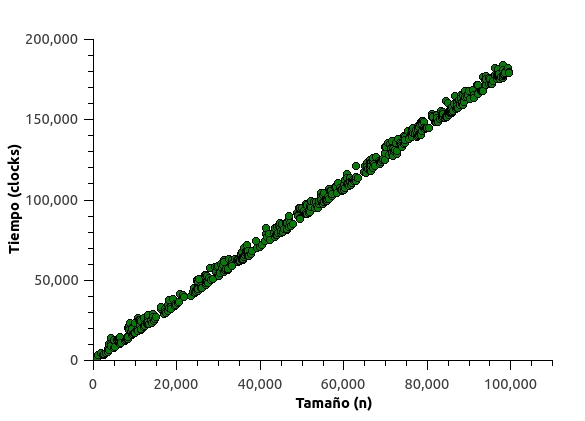
\includegraphics[scale=0.66]{imagenes/grafico1-1.jpg}
  \end{center}
\end{figure}

Si al tiempo medido lo dividimos por $log(n)$, se obtiene el siguiente resultado: 

\begin{figure}[H]
  \begin{center}
   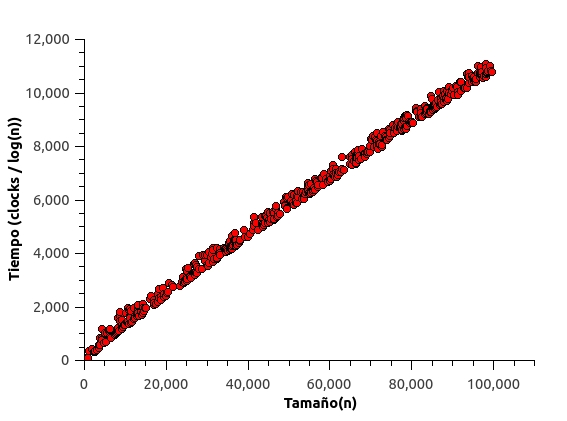
\includegraphics[scale=0.66]{imagenes/grafico1-2.jpg}
  \end{center}
\end{figure}

\newpage

Por ultimo, dividimos el ultimo resultado obtenido por $n$, para de esta manera constatar que la complejidad experimental coincide con la calculada teóricamente:

\begin{figure}[H]
  \begin{center}
   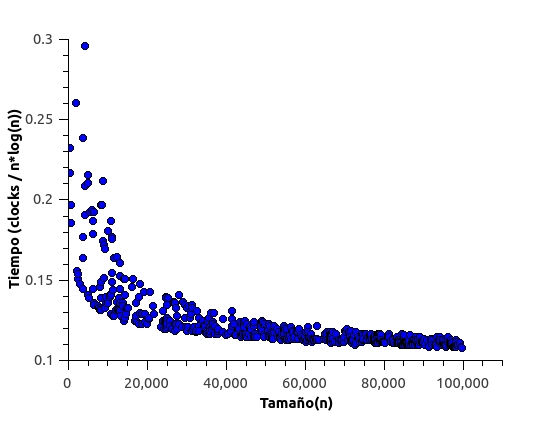
\includegraphics[scale=0.66]{imagenes/grafico1-3.jpg}
  \end{center}
\end{figure}

A continuación, adjuntamos una tabla con los últimos 20 valores obtenidos en las instancias aleatorias, teniendo en cuenta que los casos fueron previamente ordenados según el tamaño ($n$):

\begin{table}[H]
\parbox{0.3\textwidth}{
    \begin{tabular}{ | l | l |l | l |}
    \hline
	Tamaño($n$) & Tiempo($t$) & \textbf{$t / log(n)$} & \textbf{$t / n*log(n)$} \\ \hline
96,553	&	178,384	&	10,772.61	&	0.112	\\ \hline
96,631	&	176,000	&	10,627.89	&	0.110	\\ \hline
96,703	&	181,731	&	10,973.25	&	0.113	\\ \hline
96,714	&	176,870	&	10,679.63	&	0.110	\\ \hline
96,750	&	178,210	&	10,760.19	&	0.111	\\ \hline
96,998	&	177,114	&	10,691.63	&	0.110	\\ \hline
97,107	&	179,106	&	10,810.82	&	0.111	\\ \hline
97,288	&	175,469	&	10,589.58	&	0.109	\\ \hline
97,538	&	176,710	&	10,662.09	&	0.109	\\ \hline
97,904	&	176,177	&	10,626.46	&	0.109	\\ \hline
98,066	&	184,153	&	11,105.95	&	0.113	\\ \hline
98,068	&	177,755	&	10,720.08	&	0.109	\\ \hline
98,100	&	181,413	&	10,940.38	&	0.112	\\ \hline
98,229	&	178,379	&	10,756.18	&	0.110	\\ \hline
98,296	&	178,935	&	10,789.07	&	0.110	\\ \hline
98,404	&	180,022	&	10,853.57	&	0.110	\\ \hline
98,612	&	179,711	&	10,832.83	&	0.110	\\ \hline
99,097	&	182,861	&	11,018.01	&	0.111	\\ \hline
99,342	&	179,873	&	10,835.65	&	0.109	\\ \hline
99,482	&	179,194	&	10,793.42	&	0.108	\\ \hline
    \textbf{Promedio} & & & 0.110 \\ \hline

    \end{tabular}
%   \caption*{Ver Apendice A para Tabla com-pleta}
}
\end{table}

\textbf{Promedio de las 500 instancias}: 0.125
\\
\\
A partir de la información suministrada, podemos concluir que, en el último resultado, estamos en presencia de una constante cercana a 0, pero distinta a 0. Si bien esta conclusión no es suficiente como demostración matemática de que el limite no tiende a 0, si efectivamente tiende a 0, esto no afecta la conclusión a la que arribamos, ya que la complejidad sigue siendo $\mathcal{O}(n*log(n))$
De este análisis se desprende que la complejidad calculada teóricamente coincide con la complejidad de la experimentación.


\subsubsection{Experimentación con instancias particulares}
La diferencia entre mejor o peor caso viene dado por el algoritmo de ordenamiento, ya que es la operación con mayor complejidad, $\mathcal{O}(n*log(n))$. En la implementación presentada se utiliza la función   \texttt{std::sort}\footnote{Referencia:  \url{http://en.cppreference.com/w/cpp/algorithm/sort}}, que acorde a la documentación disponible\footnote{Referencia:  \url{https://gcc.gnu.org/onlinedocs/libstdc++/libstdc++-html-USERS-4.4/a01027.html}}, la complejidad es siempre la misma. Por lo cual carece de sentido plantear mejor y peor caso, ya que el resultado sería el mismo.

Para demostrar este argumento, planteamos el siguiente experimento:
\begin{itemize}
	\item Casos donde las ciudades ya están ordenadas desde el input, según el costo de salvar cada ciudad de forma creciente (posible ``mejor'' caso). Para generar este tipo de input, fijamos la cantidad de soldados y costo de enviar refuerzos de cada ciudad, mientras vamos incrementando de ciudad en ciudad los zombis en las mismas de forma que necesitamos cada vez mas soldados para rescatar la ciudad.
    \begin{codesnippet}
Ejemplo:
5 ciudades, $ XX presupuesto (es irrelevante)
ciudad 1: 1000 zombis 100 soldados $ 10 costo p/soldado
ciudad 2: 2000 zombis 100 soldados $ 10 costo p/soldado
ciudad 3: 3000 zombis 100 soldados $ 10 costo p/soldado
ciudad 4: 4000 zombis 100 soldados $ 10 costo p/soldado
ciudad 5: 5000 zombis 100 soldados $ 10 costo p/soldado
\end{codesnippet}
	\item Casos donde las ciudades ya están ordenadas desde el input, según el costo de salvar cada ciudad de forma decreciente (posible ``peor'' caso). Para generar este tipo de input, fijamos la cantidad de soldados y costo de enviar refuerzos de cada ciudad, mientras vamos decrementando de ciudad en ciudad los zombis en las mismas de forma que necesitamos cada vez menos soldados para rescatar la ciudad.

\begin{codesnippet}
Ejemplo:
5 ciudades, $ XX presupuesto (es irrelevante)
ciudad 1: 5000 zombis 100 soldados $ 10 costo p/soldado
ciudad 2: 4000 zombis 100 soldados $ 10 costo p/soldado
ciudad 3: 3000 zombis 100 soldados $ 10 costo p/soldado
ciudad 4: 2000 zombis 100 soldados $ 10 costo p/soldado
ciudad 5: 1000 zombis 100 soldados $ 10 costo p/soldado
\end{codesnippet}
    \item 100 instancias de cada tipo.
\end{itemize}

A continuación exponemos gráficamente el resultado de la experimentación:

\begin{figure}[H]
        \centering
        \begin{subfigure}[b]{0.5\textwidth}
                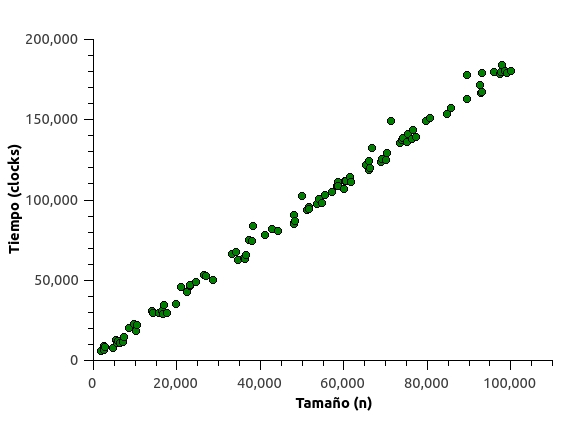
\includegraphics[width=\textwidth]{imagenes/grafico1-mejor1.jpg}
                \caption{Mejor Caso}
        \end{subfigure}%
        ~ %add desired spacing between images, e. g. ~, \quad, \qquad, \hfill etc.
          %(or a blank line to force the subfigure onto a new line)
        \begin{subfigure}[b]{0.5\textwidth}
                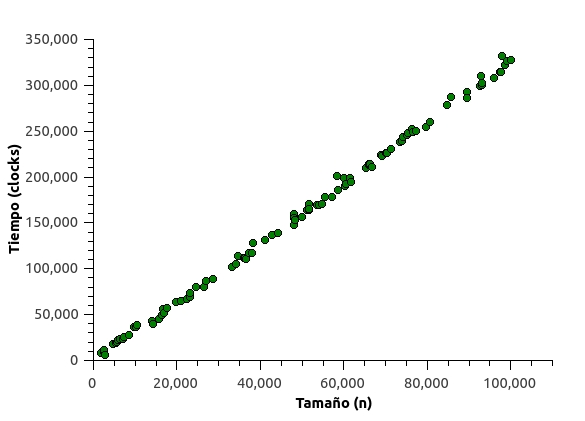
\includegraphics[width=\textwidth]{imagenes/grafico1-peor1.jpg}
                \caption{Peor Caso}
        \end{subfigure}

\end{figure}

Al igual que en el caso de las instancias aleatorias, dividimos por $log(n)$ a los tiempos obtenidos:

\begin{figure}[H]
        \centering
        \begin{subfigure}[b]{0.5\textwidth}
                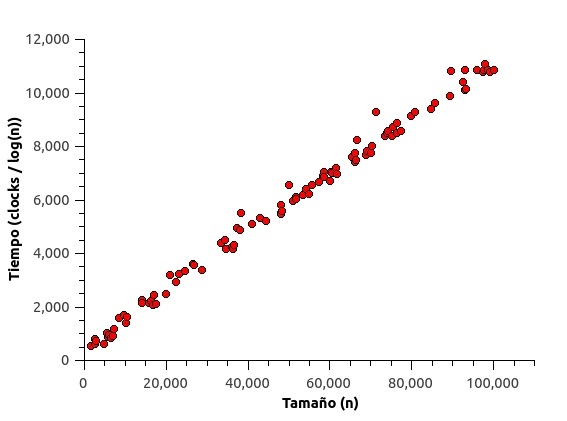
\includegraphics[width=\textwidth]{imagenes/grafico1-mejor2.jpg}
                \caption{Mejor Caso}
        \end{subfigure}%
        ~ %add desired spacing between images, e. g. ~, \quad, \qquad, \hfill etc.
          %(or a blank line to force the subfigure onto a new line)
        \begin{subfigure}[b]{0.5\textwidth}
                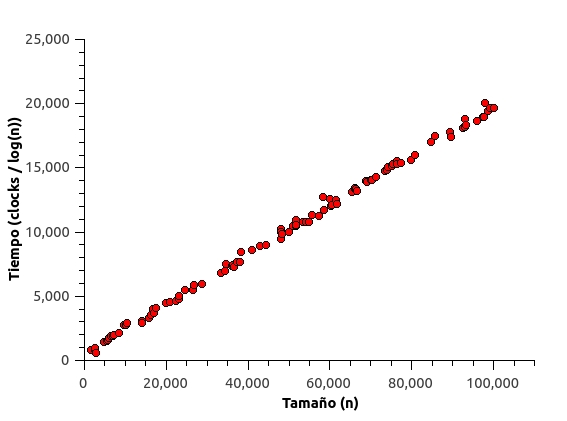
\includegraphics[width=\textwidth]{imagenes/grafico1-peor2.jpg}
                \caption{Peor Caso}
        \end{subfigure}

\end{figure}

Por último dividimos el anterior resultado por $n$:

\begin{figure}[H]
        \centering
        \begin{subfigure}[b]{0.5\textwidth}
                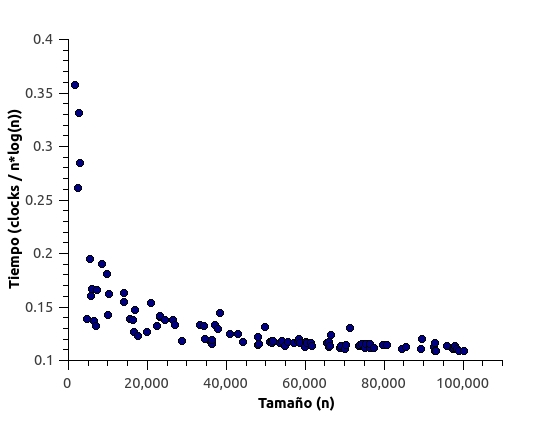
\includegraphics[width=\textwidth]{imagenes/grafico1-mejor3.jpg}
                \caption{Mejor Caso}
        \end{subfigure}%
        ~ %add desired spacing between images, e. g. ~, \quad, \qquad, \hfill etc.
          %(or a blank line to force the subfigure onto a new line)
        \begin{subfigure}[b]{0.5\textwidth}
                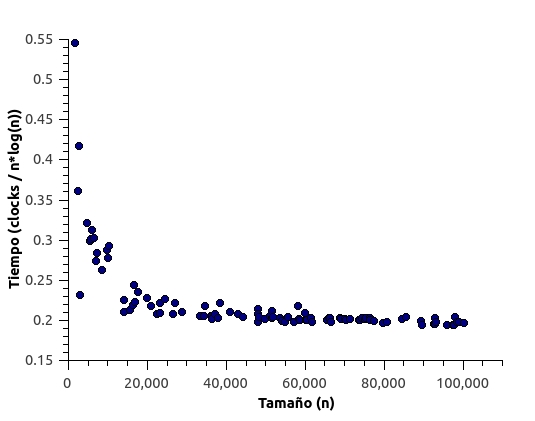
\includegraphics[width=\textwidth]{imagenes/grafico1-peor3.jpg}
                \caption{Peor Caso}
        \end{subfigure}

\end{figure}

Visualmente queda en evidencia la similitud entre ambos casos y el resultado obtenido con las instancias aleatorias. De esta forma, demostramos la inexistencia de un mejor o peor caso práctico.

A continuación, adjuntamos una tabla con los últimos 20 valores obtenidos en las instancias consideradas ``mejor''  caso, teniendo en cuenta que los casos fueron previamente ordenados según el tamaño ($n$):

\begin{table}[H]
\parbox{0.3\textwidth}{
    \begin{tabular}{ | l | l |l | l |}
    \hline
	Tamaño($n$) & Tiempo($t$) & \textbf{$t / log(n)$} & \textbf{$t / n*log(n)$} \\ \hline
75,298	&	141,520	&	8,735.63	&	0.116	\\ \hline
76,191	&	138,505	&	8,540.55	&	0.112	\\ \hline
76,329	&	144,175	&	8,888.75	&	0.116	\\ \hline
77,184	&	139,809	&	8,611.04	&	0.112	\\ \hline
79,597	&	149,414	&	9,177.52	&	0.115	\\ \hline
80,640	&	151,454	&	9,292.11	&	0.115	\\ \hline
84,521	&	154,040	&	9,411.61	&	0.111	\\ \hline
85,486	&	157,776	&	9,630.24	&	0.113	\\ \hline
89,272	&	163,195	&	9,923.13	&	0.111	\\ \hline
89,483	&	178,221	&	10,834.55	&	0.121	\\ \hline
92,479	&	171,924	&	10,421.63	&	0.113	\\ \hline
    \end{tabular}
  \caption*{Tabla 1/2}
}
\end{table}
\begin{table}[H]
\parbox{0.3\textwidth}{
    \begin{tabular}{ | l | l |l | l |}
    \hline
	Tamaño($n$) & Tiempo($t$) & \textbf{$t / log(n)$} & \textbf{$t / n*log(n)$} \\ \hline

92,854	&	167,048	&	10,122.48	&	0.109	\\ \hline
92,877	&	179,340	&	10,867.09	&	0.117	\\ \hline
93,021	&	167,888	&	10,171.78	&	0.109	\\ \hline
95,888	&	180,248	&	10,891.73	&	0.114	\\ \hline
97,401	&	179,004	&	10,801.82	&	0.111	\\ \hline
97,567	&	180,332	&	10,880.35	&	0.112	\\ \hline
97,863	&	184,156	&	11,108.14	&	0.114	\\ \hline
98,415	&	180,447	&	10,879.09	&	0.111	\\ \hline
98,914	&	179,276	&	10,803.74	&	0.109	\\ \hline
100,032	&	180,844	&	10,887.59	&	0.109	\\ \hline
    \textbf{Promedio} & & & 0.113 \\ \hline

    \end{tabular}
  \caption*{Tabla 2/2}
}
\end{table}
\textbf{Promedio de las 100 instancias}: 0.133
\\
\\
La información de los últimos 20 valores obtenidos en las instancias consideradas ``peor'' caso son:

\begin{table}[H]
\parbox{0.3\textwidth}{
    \begin{tabular}{ | l | l |l | l |}
    \hline
	Tamaño($n$) & Tiempo($t$) & \textbf{$t / log(n)$} & \textbf{$t / n*log(n)$} \\ \hline
75,298	&	248,304	&	15,327.10	&	0.204	\\ \hline
76,191	&	252,415	&	15,564.52	&	0.204	\\ \hline
76,329	&	249,327	&	15,371.63	&	0.201	\\ \hline
77,184	&	250,608	&	15,435.32	&	0.200	\\ \hline
79,597	&	254,918	&	15,657.94	&	0.197	\\ \hline
80,640	&	261,103	&	16,019.37	&	0.199	\\ \hline
84,521	&	279,177	&	17,057.29	&	0.202	\\ \hline
85,486	&	287,561	&	17,551.97	&	0.205	\\ \hline
89,272	&	293,204	&	17,828.37	&	0.200	\\ \hline
89,483	&	286,589	&	17,422.54	&	0.195	\\ \hline
92,479	&	299,692	&	18,166.63	&	0.196	\\ \hline
92,854	&	310,673	&	18,825.61	&	0.203	\\ \hline
92,877	&	300,995	&	18,238.77	&	0.196	\\ \hline
93,021	&	303,404	&	18,382.25	&	0.198	\\ \hline
95,888	&	309,010	&	18,672.36	&	0.195	\\ \hline
97,401	&	314,691	&	18,989.72	&	0.195	\\ \hline
97,567	&	315,383	&	19,028.66	&	0.195	\\ \hline
97,863	&	332,936	&	20,082.43	&	0.205	\\ \hline
98,415	&	322,493	&	19,443.00	&	0.198	\\ \hline
98,914	&	327,398	&	19,730.04	&	0.199	\\ \hline
100,032	&	327,654	&	19,726.19	&	0.197	\\ \hline
    \textbf{Promedio} & & & 0.199 \\ \hline

    \end{tabular}
%   \caption*{Ver Apendice A para Tabla com-pleta}
}
\end{table}

\textbf{Promedio de las 100 instancias}: 0.223
\\
\\


% \begin{figure}[H]
%   \begin{center}
%    \includegraphics[scale=0.66]{imagenes/grafico2-1.png}
%   \end{center}
% \end{figure}


